% Chapter Template

\chapter{Background CFD} % Main chapter title

\label{cfdintro} % Change X to a consecutive number; for referencing this chapter elsewhere, use \ref{ChapterX}

\section{Governing equations}

Governing equations tell us the rate of change for certain variables of interest, given other variables.

The governing equations we are concerned with in this project are those that concern the 3-dimensional flow and heat transfer of a newtonian compressible fluid. They are derived from the Navier-Stokes equations, which in turn are derived from simple laws of physics, like the conservation of mass, Newton's second law (F=ma) and the first law of thermodynamics (the rate of change of energy is equal to the sum of the rate of heat addition to and the rate of work done on a fluid particle).

Ours is a marching problem, where we start with initial values in a grid and iteratively change the values in each cell until we have reached time $t_{end}$

There are in total 5 balance equations we are concerned with, conserving the mass, x-momentum, y-momentum, z-momentum and energy of a fluid:

\begin{figure}[h]
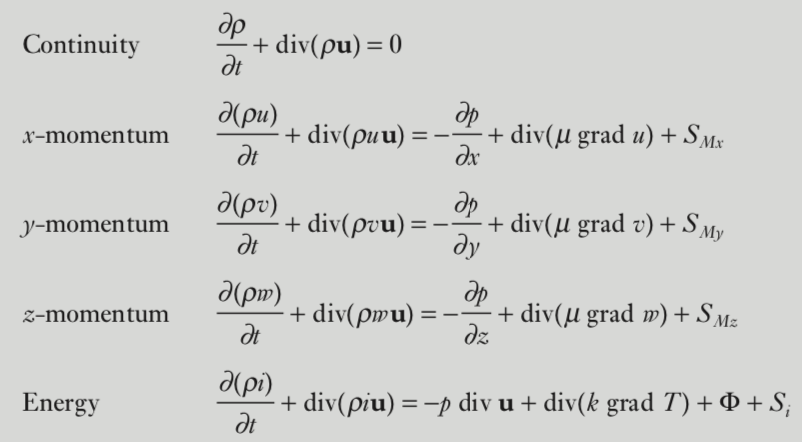
\includegraphics[scale=0.8]{5eq}
\end{figure}

$\rho = density$ \\
$t = time$ \\
$\mathbf{u} = flow vector$\\
$u = flow component in x-direction$ \\
$p = pressure$ \\
$\mu = dynamic viscosity$\\
$S_{Mx} = x-momentum source$ \\
$v = flow component in y-direction$ \\
$S_My = y-momentum source$ \\
$w = flow component in z-direction$ \\
$S_mz = z-momentum source$ \\
$i = internal energy$ \\
$k = thermal conductivity$ \\
$\Phi = dissipation function$ \\
$S_i = internal energy source$

(I don't know yet how to get space characters in functions)

Altogether we have 7 equations and 7 unknowns, giving us a closed system which can then be solved, initial and boundary conditions.

\subsection{Dissipation equation}

\begin{figure}[h]
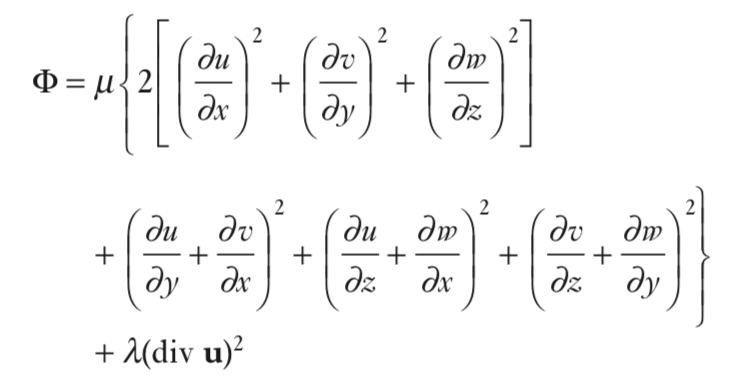
\includegraphics[scale=0.8]{dissipation}
\end{figure}
$\lambda = 2/3\mu$\\

\subsection{Equations of state}

The variables p and i  can be expressed as functions of density $\rho$ and temperature T. These functions are called the equations of state. In this project we will use an approximation where we use the ideal gas law as our equations of state:

$p = \rho RT$  and $i = C_{vT}$

$R = ideal gas constant$
$C_v = heat capacity$

Equation states assume thermodynamic equilibrium, i.e. that changes in temperature are slow enough that no significant temperature gradients appear throughout the model space.

Since we are dealing with air at low velocities, we will also assume incompressibility for our fluid. This allows us to decouple pressure (p) and density ($\rho$) so that density varies only due to temperature. 

\subsection{Continuity equation}

The continuity equation, also called the mass balance equation, is based off of conservation of mass (density in this case, since we're dealing with fixed volumes). It states that the change of mass in a volume is equal to the mass entering/leaving it via the flow.

\subsection{Momentum equations}

The three momentum equations in the x, y and z direction tell us that the rate of change in momentum in a certain direction in a volume is given by the momentum in that direction from fluid flowing into/out of the volume + the momentum in that direction given by pressure (the minus sign comes from pressure pushing in the opposite direction of its gradient) + the momentum in that direction applied by shear stresses + momentum in that direction applied by sources.

\subsection{Energy equation}

The energy equation tells us that the change rate of internal energy in a volume is equal to the internal energy from fluid flowing into/out of the volume + the potential energy from pressure it recieves/loses due to flow + the energy it recieves/loses due to thermal conductivity + the energy gained from deformation of the fluid converted into internal energy + energy from sources.

Gravity will be incorporated as an internal energy-source.

If the fluid is incompressible, $\rho$ and $i$ are uniform in space and div($\mathbf{u}$) = 0. This, together with the ideal gas law, allows us to simplify the energy equation into:

\begin{figure}[h]
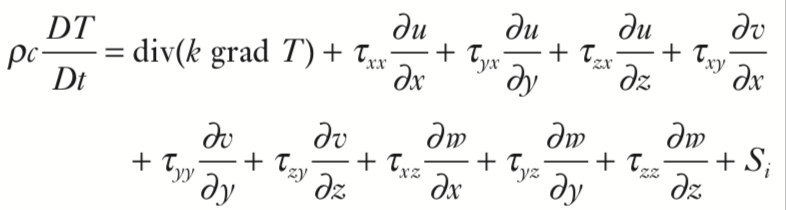
\includegraphics[scale=0.8]{newenergy}
\end{figure}

(the $\rho$ should be within the derivative since it in our case is time dependent. This allows use to convert $\rho T$ into p/R. Since we assume p is constant, its derivative over time will be 0 which means we get a left side that's 0)

\section{Transport equation}

Since we already have enough information to solve the flow of our model, we can now calculate the rate of change for specific attributes $\phi$ in the flow, through so-called transport equations.

\begin{figure}[h]
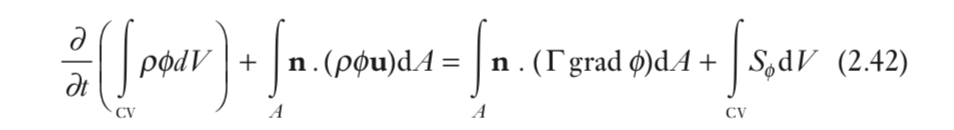
\includegraphics[scale=0.8]{navier}
\end{figure}

This equation says is that the $\phi$ gained in a unit volume $\phi$ leaving the unit volume through advection equals the $\phi$ entering the unit volume through diffusion plus the $\phi$ generated within the volume.

The same equation but time-dependent:
\\
\begin{figure}[h]
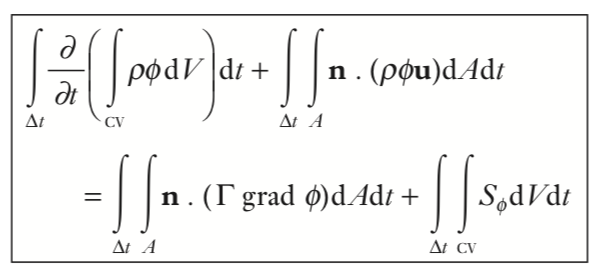
\includegraphics[scale=0.8]{naviertime}
\end{figure}
\\

Phi in our cases will be the species concentration of different chemical compounds found in an urban street environment.

\section{Turbulence}

\section{Radiation}

Radiation is the transmission of energy between bodies through space in the form of electromagnetic waves. No medium is required for this, which is why the radiative rays from the sun are able to reach the earth, despite there being no medium inbetween.

For a given body, incident radiative energy is either absorbed, reflected or transmitted, according to its \textbf{absorptivity} (a), \textbf{reflexivity} (r) and \textbf{transmissivity} ($\tau$) coefficients. These range from 0 to 1, and and have a sum equal to 1 due to the law of conservation of energy.

In most CFD cases, including this one, all boundary surfaces are opaque, meaning $\tau = 0$.

The equation for how much energy a radiative body emits is given by the Stefan-Boltzmann law:
\\
$j_r = A\epsilon \sigma_{SB}T^4$

A is the area of the body.

$\epsilon$ is the \textbf{emissivity} of the body. It is defined as the fraction of energy radiated from the body compared to the amount of energy that would be radiated by an ideal blackbody of equal surface area.

$\sigma$ is \textbf{Stefan-Boltzmann's constant}, defined as approximately $5.67*10^{-8}Wm^{-2}K^{-4}$.

T is the temperature of the body.

We can now set up an equation for the radiative energy contribution in a system:

$Sh()=aG-(\epsilon \sigma_{SB}T^4)$

Where G is equal to the incident radiative energy.

In other words, the radiatiative energy contribution to the energy equation is equal to the absorbed radiative energy (aG) minus the emitted radiative energy $(\epsilon \sigma_{SB}T^4)$. Looking at the energy equation function, this contribution can be found in the radiation->Sh(thermo) term.

\begin{verbatim}
     fvScalarMatrix hEqn(    
     fvm::div(phi, h)       
     - fvm::Sp(fvc::div(phi), h)
     - fvm::laplacian(turbulence->alphaEff(), h)      
     == fvc::div(phi/fvc::interpolate(rho)*fvc::interpolate(p))
     - p*fvc::div(phi/fvc::interpolate(rho))
     + radiation->Sh(thermo));
\end{verbatim}

To be able to solve the radiation contribution equation, the absorbptivity, emissivity and incident radiation G need to be modelled.

Absorbptivity and emissivity for a surface depend on wavelength, temperature and material. OpenFOAM has multiple functions to choose from, but for most intents and purposes a constant absoptivity/emissivity model suffices. The model can be set using the absorptionEmissionModel parameter in the \textbf{constant/radiationProperties} file.

G is trickier to model. The most widely used models are \textbf{S2S}, \textbf{FvDOM} and \textbf{P1}. They each implement the \textbf{Ru()} and \textbf{Rp()} functions, which are the constant and temperature-varying contributions to \textbf{Sh()}, respectively. We can see their use the in the \textbf{radiationModel::Sh()} function:

\begin{verbatim}
Foam::tmp<Foam::fvScalarMatrix> Foam::radiation::radiationModel::Sh
 (
     const basicThermo& thermo,
     const volScalarField& he
 ) const
 {
     const volScalarField Cpv(thermo.Cpv());
     const volScalarField T3(pow3(T_));
  
     return
     (
         Ru()
       - fvm::Sp(4.0*Rp()*T3/Cpv, he)
       - Rp()*T3*(T_ - 4.0*he/Cpv)
     );
 }
\end{verbatim}

The equation looks complicated at first glance, but the fvm::Sp() row and parts of the third row are simply an addition and subtraction of the same term in order to increase diagonal dominance. It's made more clear with the shifting of some terms:

$Sh() = Ru() - (4Rp*\frac{T^3h}{C_p}) - Rp()T^4 + (4Rp*\frac{T^3h}{C_p}) = Ru() - Rp()T^4$

The radiation models will in different ways calculate Ru() and Rp() in a way that makes Sh() represent our analytically derived $aG-(\epsilon \sigma_{SB}T^4)$ equation.

\subsection{viewFactor}

The viewFactor model calculates, for each boundary face of the mesh, a view factor coefficient for each other face in the mesh, determined by how "visible" the faces are to each other. The incident radiation for a face is then calculated by adding together the emitted radiative energy of all faces visible to that face, weighted by their view factor.

It assumes full transparency for the fluid and therefore gives no actual direct contribution to the radiation term of the energy equation. Instead it calculates qr, the boundary heat flux of the boundary patches, to be used in boundary condition equations of the mesh. In this way radiative energy is added to a cell through the $\nabla (\Gamma \nabla T)$ term rather than the radiationModel.Sh(thermo) term. The wall is only evaluated at the faces of the mesh. The model requires a lot of memory space to store the view factors, especially for finer meshes.

\subsection{FvDOM}

The FvDOM (Finite volume Discrete Ordinates Model) model divides emitted rays into a discrete number of solid angles, and solves them through ray-tracing. It is a computationally expensive but accurate radiation model.

\subsection{P1}

The P1 model simply assumes directional equilibrium between rays, and solves for the incident radiation as if it were a diffusive attribute. It works best for cases where the optical thickness (a * L) is high, i.e. where a substantial fraction of a beam's energy gets absorbed by the fluid before reaching a boundary.

It uses the following transport equation for G:

$\nabla * (\Gamma \nabla G) - aG + 4\epsilon \sigma T^4$

Which can found in the P1.C file as:

\begin{verbatim}
// Solve G transport equation
solve
(
    fvm::laplacian(gamma, G_)
    - fvm::Sp(a_, G_)
    ==
    - 4.0*(e_*physicoChemical::sigma*pow4(T_) ) - E_
);
\end{verbatim}

Here, \textbf{e\_} is the emmissivity, \textbf{sigma} is the Stefan-Boltzmann constant and \textbf{E\_} is the emission contribution.

Gamma is the "diffusive" coefficient for the P1 radiation, and is calculated in the following function:

\begin{verbatim}
// Construct diffusion
const volScalarField gamma
(
    IOobject
    (
        "gammaRad",
        G_.mesh().time().timeName(),
        G_.mesh(),
        IOobject::NO_READ,
        IOobject::NO_WRITE
    ),
    1.0/(3.0*a_ + sigmaEff + a0)
);
\end{verbatim}

here sigmaeff represents the scattering coefficient, which tells us how much ray intensity fades for each unit length travelled through the fluid.

\section{Solar load}

The solarLoad library, implemented for OpenFOAM+, is used to calculate the solar load on a CFD mesh. The direction of the sunbeams is set either to a constant direction or calculated with the included solarCalculator class. It also accounts for shading and reflexivity.

It can either act as a standalone radiation model or be added onto the viewFactor and FvDOM radiation models by setting \textbf{useSolarLoad} to \textbf{true} in \textbf{constant/radiationProperties}. The parameters for your solar model are then set in the \textbf{solarLoadCoeffs} dictionary in the same file. If combining solarLoad with FvDOM, you can only use one frequency band in the domain. When using the solarLoad model in conjunction with another model, it is only evaluated at boundary faces, not the internal field (similar to viewFactor).

\subsection{solarLoad.C}

Looking at solarLoad.C's Rp() function:

\begin{verbatim}
Foam::tmp<Foam::volScalarField> Foam::radiation::solarLoad::Rp() const
{
    return tmp<volScalarField>::New
    (
        IOobject
        (
            "Rp",
            mesh_.time().timeName(),
            mesh_,
            IOobject::NO_READ,
            IOobject::NO_WRITE,
            false
        ),
        mesh_,
        dimensionedScalar
        (
            dimMass/pow3(dimTime)/dimLength/pow4(dimTemperature),
            Zero
        )
    );
}
\end{verbatim}
We can see that its Rp() function returns zero. This is because the Rp() coefficient represents the part of the radiation contribution that scales with $T^4$. Since the sun's intensity depends on the sun and not on the temperatures within the mesh, the solarLoad model only contributes to the Ru() part of Sh().

The Ru value is calculated with the calculate() function:
\begin{verbatim}
void Foam::faceShading::calculate()
{

...

bool facesChanged = updateHitFaces();

...

updateDirectHitRadiation(hitFacesId, includeMappedPatchBasePatches);

...

updateSkyDiffusiveRadiation
        (
            includePatches,
            includeMappedPatchBasePatches
        );

...

if (useReflectedRays_)
        {
            updateReflectedRays(includeMappedPatchBasePatches);
        }
        
...

}
\end{verbatim}

It calls on 4 sub-functions, described below.

\subsubsection{updateHitFaces()}

This sub-function recalculates the sun's position and subsequently determines the boundary faces that are directly hit by sunlight based on the new position by calling hitFaces\_->correct(). The hit faces are stored in the hitFaces\_ object, which is an instance of the class faceShading, defined in faceShading.C.

\begin{verbatim}
bool Foam::radiation::solarLoad::updateHitFaces()
{

    ...
    
        if (updateIndex > updateTimeIndex_)
        {
            Info << "Updating Sun position..." << endl;
            updateTimeIndex_ = updateIndex;
            solarCalc_.correctSunDirection();
            hitFaces_->direction() = solarCalc_.direction();
            hitFaces_->correct();
            return true;
        }
        
    ...    
        
}
\end{verbatim}
\begin{verbatim}
void Foam::faceShading::correct()
{
    calculate();
}
\end{verbatim}
\begin{verbatim}
void Foam::faceShading::calculate()
{

    ...

        if (((direction_ & nf) > 0) && (t[faceI] == 0.0))
        {
            dynFacesI.append(faceI + pp.start());
            dynCf.append(cf[faceI]);
            nFaces++;
        }

    ...
    
\end{verbatim}

First all the faces whose normal vectors have a component facing the sun, determined by (direction\_ \& nf > 0) (\& is a dot product operator in OpenFOAM), and whose transparency equal 0, are collected.

\begin{verbatim}
    
    ...
    
    scalar maxBounding = 5.0*mag(mesh_.bounds().max() - mesh_.bounds().min());
    
    ...
    
    do
        {
            for (; i < Cfs.size(); i++)
            {
                const point& fc = Cfs[i];
    
                const label myFaceId = hitFacesIds[i];
    
                const vector d(direction_*maxBounding);
    
                start.append(fc - 0.001*d);
    
                startIndex.append(myFaceId);
    
                end.append(fc - d);
    
            }
    
        }while (returnReduce(i < Cfs.size(), orOp<bool>()));
        
    ...
\end{verbatim}

Here we, for each face that was stored earlier, store its center as a start point (or rather, the point just before the sun hits the center). Then we project a vector from that point towards the sun with a magnitude of approximately 5 times the diagonal of the mesh (direction\_*maxBounding), and store the point at the other end of that vector as the corresponding end point. startIndex helps the program remember which face the points correspond to.

\begin{verbatim}

    ...
    
        List<pointIndexHit> hitInfo(startIndex.size());
            surfacesMesh.findLine(start, end, hitInfo);
    
            // Collect the rays which has 'only one not wall' obstacle between
            // start and end.
            // If the ray hit itself get stored in dRayIs
            forAll(hitInfo, rayI)
            {
                if (!hitInfo[rayI].hit())
                {
                    rayStartFace.append(startIndex[rayI]);
                }
            }
            
    ...

}
\end{verbatim}

The surfacesMesh.findLine(start, end, hitInfo) function calculates, for every start and end point pair, if the line going from the start point to the end point ever intersects the mesh, and stores that information in hitInfo. In the forAll loop that follows, every face that has an unblocked path towards the sun is stored in rayStartFace. These faces get transferred to the public list rayStartFaces\_, which can be accessed by solarLoad.C.

\subsubsection{updateDirectHitRadiation()}

This sub-function calculates the heat flux contribution from direct solar exposure.

\begin{verbatim}
bool Foam::radiation::solarLoad::updateDirectHitRadiation()
{
    
    ...

        const vector qPrim =
            solarCalc_.directSolarRad()*solarCalc_.direction();

        const vectorField& n = pp.faceNormals();

        {
            qprimaryBf[patchID][localFaceI] +=
                (qPrim & n[localFaceI])
                * spectralDistribution_[bandI]
                * absorptivity_[patchID][bandI]()[localFaceI];
        }

        if (includeMappedPatchBasePatches[patchID])
        {
            qrBf[patchID][localFaceI] += qprimaryBf[patchID][localFaceI];
        }
        else
        {
            const vectorField& sf = mesh_.Sf().boundaryField()[patchID];
            const label cellI = pp.faceCells()[localFaceI];

            Ru_[cellI] +=
                (qPrim & sf[localFaceI])
              * spectralDistribution_[bandI]
              * absorptivity_[patchID][bandI]()[localFaceI]
              / V[cellI];
        }
\end{verbatim}

We will later find out how the solar calculator works. In the above code we can see that a vector representing sunlight, qPrim, is defined. It has the same direction as the sun, and the same magnitude as the solar intensity (directSolarRad()). Then, for each frequency band, each face of each patch gets added to it a heat flux value (qprimaryBf), equal to the dot product between the sun and the face normal, times the normalized spectral distribution of that band, times the absorptivity of that face for that band. The reason why a dot product with the face normal is used as a factor is to account for the angular visibility of the face.

The calculated flux then gets added either to the qr\_ variable (which qrBf references) or to the energy equation of the cells next to the walls, depending on settings set in the case files.

\subsubsection{updateSkyDiffusiveRadiation()}

This sub-function calculates the sky diffusive radiation contribution, which represents the radiation absorbed by the atmosphere and ground and then re-emitted in a diffuse manner throughout the mesh.

It is calculated differently depending on the solar model used. 

\begin{verbatim}
void Foam::radiation::solarLoad::updateSkyDiffusiveRadiation
(
    const labelHashSet& includePatches,
    const labelHashSet& includeMappedPatchBasePatches
)
{
    const polyBoundaryMesh& patches = mesh_.boundaryMesh();
    const scalarField& V = mesh_.V();
    volScalarField::Boundary& qrBf = qr_.boundaryFieldRef();

    switch(solarCalc_.sunLoadModel())
    {
        case solarCalculator::mSunLoadFairWeatherConditions:
        case solarCalculator::mSunLoadTheoreticalMaximum:
        {
            for (const label patchID : includePatches)
            {
                const polyPatch& pp = patches[patchID];
                const scalarField& sf = mesh_.magSf().boundaryField()[patchID];

                const vectorField n = pp.faceNormals();
                const labelList& cellIds = pp.faceCells();

                forAll(n, faceI)
                {
                    const scalar cosEpsilon(verticalDir_ & -n[faceI]);

                    scalar Ed(0.0);
                    scalar Er(0.0);
                    const scalar cosTheta(solarCalc_.direction() & -n[faceI]);

                    {
                        // Above the horizon
                        if (cosEpsilon == 0.0)
                        {
                            // Vertical walls
                            scalar Y(0);

                            if (cosTheta > -0.2)
                            {
                                Y = 0.55+0.437*cosTheta + 0.313*sqr(cosTheta);
                            }
                            else
                            {
                                Y = 0.45;
                            }
                            Ed = solarCalc_.C()*Y*solarCalc_.directSolarRad();
                        }
                        else
                        {
                            //Other than vertical walls
                            Ed =
                                solarCalc_.C()
                              * solarCalc_.directSolarRad()
                              * (1.0 + cosEpsilon)/2.0;
                        }

                        // Ground reflected
                        Er =
                            solarCalc_.directSolarRad()
                          * (solarCalc_.C() + Foam::sin(solarCalc_.beta()))
                          * solarCalc_.groundReflectivity()
                          * (1.0 - cosEpsilon)/2.0;
                    }

                    const label cellI = cellIds[faceI];
                    if (includeMappedPatchBasePatches[patchID])
                    {
                        for (label bandI = 0; bandI < nBands_; bandI++)
                        {
                            qrBf[patchID][faceI] +=
                                (Ed + Er)
                              * spectralDistribution_[bandI]
                              * absorptivity_[patchID][bandI]()[faceI];
                        }
                    }
                    else
                    {
                        for (label bandI = 0; bandI < nBands_; bandI++)
                        {
                            Ru_[cellI] +=
                                (Ed + Er)
                              * spectralDistribution_[bandI]
                              * absorptivity_[patchID][bandI]()[faceI]
                              * sf[faceI]/V[cellI];
                        }
                    }
                }
            }
        }
        break;
    }
\end{verbatim}

For the mSunLoadFairWeatherConditions and mSunLoadTheoreticalMaximum models, the model creates a cosEpsilon value for each face, being the dot product between the reversed face normal and the vector pointing towards the earth's core (in almost every case, the normalized g vector). Since both the reversed normal vector and the downwards pointing vector are normalized, the dot product will be equal to the cosine of the angle between them. This means that a face on the floor, whose reversed normal vector points downwards, will get the cosEpsilon value of cos(0) = 1. A vertical wall face, whose normal (and reverse normal) will always be at a 90 degree angle from the g vector, giving the face a cosEpsilon value of cos(90) = 0. Non-orthogonal faces will have a value inbetween 0 and 1. An exception to this are faces with a normal vector with a downwards facing component, which have a cosEpsilon value of [-1, 0).

Each face then gets assigned an Ed and an Er value, which each represent the diffusive radiance contribution from the sky and ground respectively. Their equations each feature a view factor. For sky diffusivity it equals (1.0 - cosEpsilon)/2.0 and ground for ground diffusivity it equals (1.0 - cosEpsilon)/2.0. They both range from 0 to 1, and add up to 1 for any one face. They can be seen as angle-dependent weights for a face. A face on the floor will have a ground diffusivity wieght of 0 and a sky diffusivity of 1, since it can only see the sky and not the ground.

Vertical faces get special treatment. Faces where cosTheta > -0.2, i.e. where the normal vector points somewhat away from the sun, i.e. significantly shaded faces, get a sky diffusive weight of 0.55+0.437*cosTheta + 0.313*sqr(cosTheta). Vertical faces somewhat pointing towards the sun are assigned a sky diffusive wieght of 0.45, slightly lower than the 0.5 they would have been assigned by the (1.0 + cosEpsilon)/2.0 function.

The diffusive radiation intensities for sky and ground diffusion are determined by the diffusive constant C, the solar intensity directSolarRad and the groundReflectivity, all defined at run-time in the solarLoadCoeffs dictionary.

The mSunLoadConstant model has a much simpler calculation:

\begin{verbatim}
        case solarCalculator::mSunLoadConstant:
        {
        
            ...
            
                {
                    for (label bandI = 0; bandI < nBands_; bandI++)
                    {
                        qrBf[patchID][faceI] +=
                            solarCalc_.diffuseSolarRad()
                          * spectralDistribution_[bandI]
                          * absorptivity_[patchID][bandI]()[faceI];
                    }
                }
                else
                {
                    for (label bandI = 0; bandI < nBands_; bandI++)
                    {
                        Ru_[cellI] +=
                            (
                                spectralDistribution_[bandI]
                              * absorptivity_[patchID][bandI]()[faceI]
                              * solarCalc_.diffuseSolarRad()
                            )*sf[faceI]/V[cellI];
                    }
                }
                
            ...   
                    
        }
    }
}
\end{verbatim}

Here, the user-defined diffusive solar irradiation intensity (diffuseSolarRad) is simply added on to walls directly in a uniform matter. The calculation is the same as in the updateDirectHitRadiation function, except there's no reduction of absorption based on the angle of exposure.

\subsubsection{updateReflectedRays()}

This sub-function calculates specular reflection with a depth of 1 bounce. It does so in a similar way to FvDOM, where only a discrete number of angles are available. Each time a bounce direction is calculated it selects the discrete angle that's as close to it as possible, and that becomes its actual direction.

\begin{verbatim}
void Foam::radiation::solarLoad::updateReflectedRays
(
    const labelHashSet& includePatches
)
{

    ...

        reflectedFaces_->correct();
        
    ...
\end{verbatim}

reflectedFaces is an instance of the faceReflecting class, defined in faceReflecting.C.

\begin{verbatim}
void Foam::faceShading::correct()
{
    calculate();
}
\end{verbatim}

\begin{verbatim}
void Foam::faceReflecting::correct()
{
    calculate();
}
\end{verbatim}

\begin{verbatim}
void Foam::faceReflecting::calculate()
{

    ...

        vector refDir =
            sunDir + 2.0*(-sunDir & n[faceI]) * n[faceI];

          // Look for the discrete direction
                    scalar dev(-GREAT);
                    label rayIndex = -1;
                    forAll(refDiscAngles_, iDisc)
    
            forAll(refDiscAngles_, iDisc)
                {
                    scalar dotProd = refDir & refDiscAngles_[iDisc];
                    if (dev < dotProd)
                    {
                        dev = dotProd;
                        rayIndex = iDisc;
                    }
                }
    
                if (rayIndex >= 0)
                {
                    if (refDisDirsIndex[rayIndex] == -1)
                    {
                        refDisDirsIndex[rayIndex] = 1;
                    }
                }
    
                refFacesDirIndex.insert
                (
                    globalNumbering.toGlobal(globalID),
                    rayIndex
                );
                        
    ...
    
\end{verbatim}

Here refDir is calculated as the exact reflection angle off the face. In the following forAll loop, each available discrete angle is gone through and compared to refDir. The angle whose dot product with refDir is the largest is stored as rayIndex. Since cos gets larger as it approaches 0, the discrete angle with the largest dot product will also have the smallest angle in reference to refDir. rayIndex then gets stored in refFacesDirIndex for later use.

\begin{verbatim}

    ...

    scalar maxBounding = 5.0*mag(mesh_.bounds().max() - mesh_.bounds().min());

    ...

        forAll(refDisDirsIndex, dirIndex)
                    {
                        if (refDisDirsIndex[dirIndex] > -1)
                        {
                            if ((nf & refDiscAngles_[dirIndex]) > 0)
                            {
                                const vector direction = -refDiscAngles_[dirIndex];
        
                                start.append(fc + 0.001*direction);
        
                                startIndex.append(myFaceId);
                                dirStartIndex.append(dirIndex);
        
                                end.append(fc + maxBounding*direction);
                            }
                        }
                    }
                }
        
            }while (returnReduce(i < Cfs_->size(), orOp<bool>()));
        
            List<pointIndexHit> hitInfo(startIndex.size());
        
            surfacesMesh_->findLine(start, end, hitInfo);
                        
    ...
    
\end{verbatim}

Here the faces hit by the reflected rays are determined in a similar way they were in updateDirectHits(), except here hitInfo isn't used to find the lines without intersections, but is instead used to find the faces it intersects with.


\subsection{solarCalculator}

The solarCalculator class keeps track of the sun direction and solar intensity. There are 2 models for direction and 3 for intensity. Direction is calculated in the calculateSundirection function, which uses the beta and theta angle variables, which are the sun angle above the horizon and the sun's cardinal angle in relation to the southern direction, respectively. These are calculated in the calculateBetaTheta function. The models for sun direction are:

\subsubsection{sunDirConstant}

Sun direction is set in the dictionary with the sunDirection entry.

\subsubsection{sunDirTracking}

Beta and theta are calculated from the following parameters:
\begin{itemize}
    \item localStandardMeridian : GMT (Local Zone Meridian) in hours
    \item startDay :  day from 1 to 365)
    \item startTime:  in hours
    \item longitude:  in degrees
    \item latitude:   in degrees
    \item gridUp:     grid orientation upwards
    \item gridEast    grid orientation eastwards
\end{itemize}
            
The parameters are specified in the solarLoadCoeffs dictionary.


As for intensity, the available models are:

\subsubsection{sunLoadConstant}

Solar intensity is set in the dictionary entries directSolarRad and diffuseSolarRad

\subsubsection{sunLoadFairWeatherConditions}

The solar intensity follows the Fair Weather Conditions Method from the ASHRAE Handbook. The entries are (taken from the comments of the source code):

\begin{itemize}
    \item skyCloudCoverFraction: Fraction of sky covered by clouds (0-1)
    \item A: Apparent solar irradiation at air mass m = 0
    \item B: Atmospheric extinction coefficient
    \item beta: Solar altitude (in degrees) above the horizontal plane. Is either entered or calculated
    \item groundReflectivity : Ground reflectivity
\end{itemize}

The direct solar flux is calculated as:

$directSolarRad = (1 - 0.75*skyCloudCoverFraction^3)*\frac{A}{exp(B/sin(beta)})$

\subsubsection{sunLoadTheoreticalMaximum}

The solar intensity is the same as for sunlight falling at a 0 degree angle with no cloud cover.

The entries are (taken from the source code comments):
\begin{itemize}
    \item Setrn
    \item SunPrime
    \item roundReflectivity
\end{itemize}
In this model the flux is calculated as: directSolarRad = Setrn*SunPrime

Sky diffusivity is calculated in the same way as in sunLoadFairWeatherConditions.

\section{Boundary conditions}

\subsection{Marshak Boundary Condition}

\subsection{externalWallHeatFluxTemperature}

